\chapter{Additional Experiment and Statistics}
\label{chap:additional_exp}
In this appendix chapter we put a series of extra experiments as well as all numeric measurements not previously shown in the results chapter.

\section{Additional Experiment: Varying CC/EV}
\label{sec:additional_cc_ev_exp}
In this experiment we examine the bahaviour of LDOF PED MC method for a varying the eigenvalue-cluster count. For 2 to 6 clusters and for 2 to 6 eigenvectors we generate segmentations on the Waving Hand dataset and plot the resulting performance (Fig. $\ref{fig:wh_altering_ev_cc_app}$. This experiment will give us some further insight about choosing appropriate eigenvalue (EV) and cluster count (CC) we want to solve for in MinCut (MC) and Spectral clustering (SC). The corresponding statistics are listed in Table $\ref{tab:wh_ev_c}$. To give the reader a easier way to understand the results we visualized the resulting statistics. For fixed cluster counts, we plotted the recall-precession and the eigenvector-f1 score graphs. Moreover, for fixed eigenvector counts we plotted the resulting recall-precession and clusters-f1 score graphs. 
\begin{figure}[H]
\begin{center}
\subfigure[Varying Clusters Recall/Precision Plot]{
   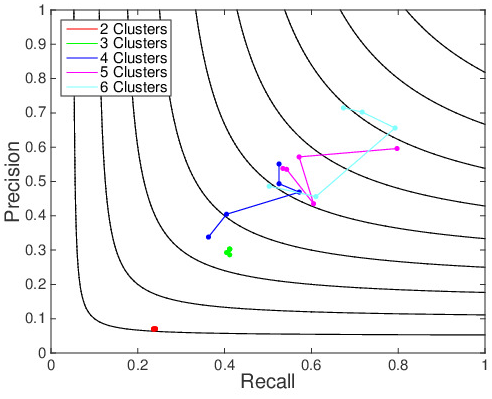
\includegraphics[width=0.47\linewidth] {evaluation/wh1/perf_ev_c/clusters_rec_prec}
}
\subfigure[Varying Clusters EV/F1 Score Plot]{
   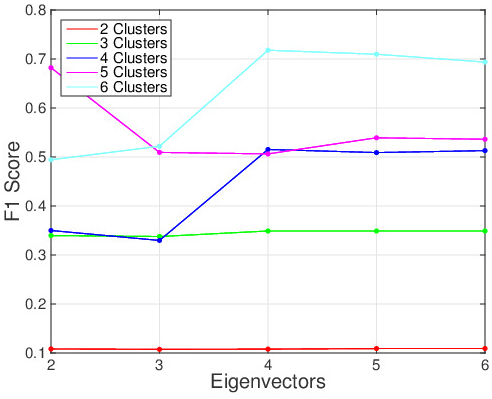
\includegraphics[width=0.47\linewidth] {evaluation/wh1/perf_ev_c/clusters_ev_f1}
}
\subfigure[Varying EV Recall/Precision Plot]{
   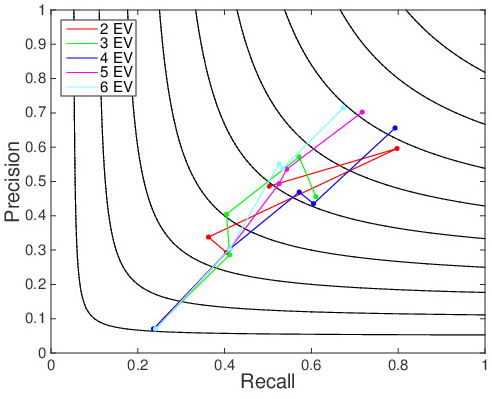
\includegraphics[width=0.47\linewidth] {evaluation/wh1/perf_ev_c/ev_rec_prec}
}
\subfigure[Varying EV Clusters/F1 Score Plot]{
   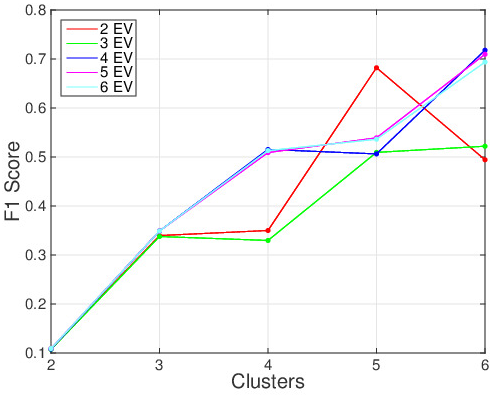
\includegraphics[width=0.47\linewidth] {evaluation/wh1/perf_ev_c/ev_c_f1}
}
\end{center}
\caption[Plot Performance Varying CLusters/Eigenvectors]{Visualizing the experiment \enquote{Varying CC/EV} via graphs: For a fixed number of eigenvectors and an altering cluster count (first row) we show the recall/precision and eigenvector/F1-Score plots. Similarly, we show recall/precision and clusters/F1-Score plots plots for a fixed number of clusters and an altering number of eigenvectors (second row). The utilized measurements for this plots is listed in Table $\ref{fig:wh_altering_ev_cc_app}$.}
\label{fig:wh_altering_ev_cc_app}
\end{figure}

\begin{table}[H]
\centering
\begin{tabular}{|l|c|c|c|c|c|}
\hline
\multicolumn{6}{|c|}{Performance Varying Eigenvectors/Clusters PED MC} \\ \hline
\multicolumn{6}{|c|}{Precision} \\ \hline
\textbf{Eigenvectors / Clusters} & 2 & 3 & 4 & 5 & 6 \\ \hline
2 & 7.03\% & 29.28\% & 33.80\% & 59.61\% & 48.63\%  \\ \hline
3 & 6.95\% & 28.62\% & 40.45\% & 57.17\% & 45.59\%  \\ \hline
4 & 6.99\% & 30.28\% & 46.90\% & 43.53\% & 65.60\%  \\ \hline
5 & 7.05\% & 30.28\% & 49.35\% & 53.55\% & 70.23\%  \\ \hline
6 & 7.05\% & 30.28\% & 50.11\% & 53.81\% & 71.47\%  \\ \hline
\multicolumn{6}{|c|}{Recall} \\ \hline
2 & 23.64\% & 40.45\% & 36.28\% & 79.73\% & 50.27\%  \\ \hline
3 & 23.64\% & 41.17\% & 40.45\% & 57.17\% & 61.04\%  \\ \hline
4 & 23.64\% & 41.17\% & 57.20\% & 60.50\% & 79.28\%  \\ \hline
5 & 24.09\% & 41.17\% & 52.55\% & 54.29\% & 71.71\%  \\ \hline
6 & 24.09\% & 41.17\% & 52.55\% & 53.42\% & 67.39\%  \\ \hline
\multicolumn{6}{|c|}{F1 Score} \\ \hline
2 & 10.83\% & 33.97\% & 35.00\% & 68.22\% & 49.43\%  \\ \hline
3 & 10.74\% & 33.77\% & 32.97\% & 50.94\% & 52.20\%  \\ \hline
4 & 10.79\% & 34.90\% & 51.54\% & 50.63\% & 71.79\%  \\ \hline
5 & 10.91\% & 34.90\% & 50.90\% & 53.92\% & 70.97\%  \\ \hline
6 & 10.91\% & 34.90\% & 51.30\% & 53.62\% & 69.37\%  \\ \hline
\end{tabular}
\caption[Performance Varying Eigenvector-Cluster]{Measurements of the experiment \enquote{Varying CC/EV} on the Waving Hand dataset (Fig. $\ref{fig:wh_altering_ev_cc_app}$).}
\label{tab:wh_ev_c}
\end{table}

\section{Varying Cluster Count on SC and MC}
This experiment should examine the behaviour of the modes PD SC, PD MC, PED SC, PED MC when using LDOF flow fields for a varying number of clusters on the One Chair dataset (Fig. $\ref{fig:chair_3_cast_dataset_appendix}$). The quantitative results are visualized in Figure $\ref{fig:chair_3_cast_plot_avg_stat}$. Additionally, qualitative results of the best resulting segmentations (Fig. $\ref{fig:chair_3_cast_best_f_score_results}$) and the worst result (Fig. $\ref{fig:chair_3_cast_gt_worst_best}$) are visualized below. The corresponding measurements of these experiments are listed in Table $\ref{tab:chair_3_cast_avg_performance}$.
\begin{figure}[H]
\begin{center}
\subfigure[Frame 30]{
   \includegraphics[width=0.31\linewidth] {evaluation/chairs_3_cast/ds/45}
}
\subfigure[Frame 45]{
   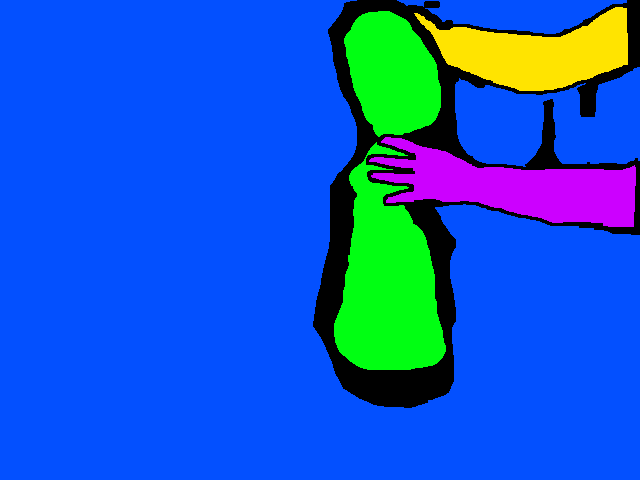
\includegraphics[width=0.31\linewidth] {evaluation/chairs_3_cast/ds/60}
}
\subfigure[Frame 60]{
   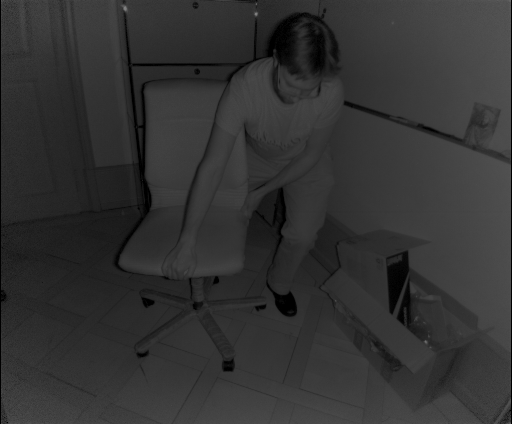
\includegraphics[width=0.31\linewidth] {evaluation/chairs_3_cast/ds/75}
}
~
\subfigure[Gt Frame 45]{
   \includegraphics[width=0.31\linewidth] {evaluation/chairs_3_cast/gt/45}
}
\subfigure[GT Frame 60]{
   \includegraphics[width=0.31\linewidth] {evaluation/chairs_3_cast/gt/60_amb}
}
\subfigure[GT Frame 75]{
   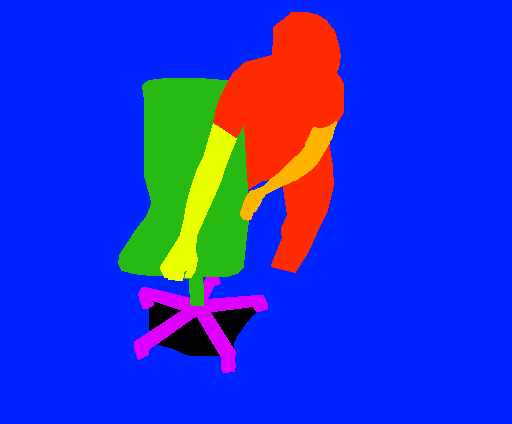
\includegraphics[width=0.31\linewidth] {evaluation/chairs_3_cast/gt/75_amb}
}
\end{center}
\caption[Chair 3 Cast Dataset]{Visualizing the ground truth frame and their frames of the One Chairs dataset}
\label{fig:chair_3_cast_dataset_appendix}
\end{figure}

\begin{figure}[H]
\begin{center}

\subfigure[Raw 5 Clusters PED MC]{
   \includegraphics[width=0.22\linewidth] {evaluation/chairs_3_cast/best/ped_mc_c_5}
}
\subfigure[5 Clusters PED MC]{
   \includegraphics[width=0.22\linewidth] {evaluation/chairs_3_cast/merged/ped_mc_c_5}
}
\subfigure[Raw 10 Clusters PED MC]{
   \includegraphics[width=0.22\linewidth] {evaluation/chairs_3_cast/best/ped_mc_c_10}
}
\subfigure[10 Clusters PED MC]{
   \includegraphics[width=0.22\linewidth] {evaluation/chairs_3_cast/merged/ped_mc_c_10}
}
~
\subfigure[Raw 15 Clusters PD SC]{
   \includegraphics[width=0.22\linewidth] {evaluation/chairs_3_cast/best/pd_sc_c_15}
}
\subfigure[15 Clusters PD SC]{
   \includegraphics[width=0.22\linewidth] {evaluation/chairs_3_cast/merged/pd_sc_c_15}
}
\subfigure[Raw 20 Clusters PD SC]{
   \includegraphics[width=0.22\linewidth] {evaluation/chairs_3_cast/best/ped_mc_c_20}
}
\subfigure[20 Clusters PED MC]{
   \includegraphics[width=0.22\linewidth] {evaluation/chairs_3_cast/merged/ped_mc_c_20}
}
\end{center}
\caption[Chair 3 Cast Winner]{Listing the four top segmentation results of frame 60 according to their scored F1 value (Tab. $\ref{tab:chair_3_cast_avg_performance})$. On the left, the unmerged- and on the right the merged segmentation.}
\label{fig:chair_3_cast_best_f_score_results}
\end{figure}

\begin{table}[H]
\centering
\begin{tabular}{|l|c|c|c|c|}
\hline
\multicolumn{5}{|c|}{Average Precision} \\ \hline
\textbf{Method / \#Cluster} & 5 & 10 & 15 & 20 \\ \hline
PD SC & 18.01\% & \textbf{55.17}\% & \textbf{55.12}\% & \textbf{56.23}\% \\ \hline
PD MC & \textbf{38.70}\% & 38.14\% & 45.65\% & 49.64\% \\ \hline
PED SC & 13.14\% & 35.29\% & 50.75\% & 52.14\%  \\ \hline
PED MC & 26.81\% & 42.94\% & 38.70\% & \textbf{56.23}\% \\ \hline
\multicolumn{5}{|c|}{Average Recall} \\ \hline
PD SC & 12.34\% & 19.22\% & 38.13\% & 47.82\% \\ \hline
PD MC & 13.10\% & 24.51\% & \textbf{44.07}\% & \textbf{53.50}\% \\ \hline
PED SC & 10.20\% & 28.29\% & 39.24\% & 33.75\% \\ \hline
PED MC & \textbf{19.37}\% & \textbf{38.86}\% & 41.88\% & 50.07\% \\ \hline
\multicolumn{5}{|c|}{Average F1 Score} \\ \hline
PD SC & 14.02\% & 28.47\% & \textbf{45.04}\% & 51.59\% \\ \hline
PD MC & 19.50\% & 29.79\% & 44.63\% & 51.40\% \\ \hline
PED SC & 11.48\% & 30.89\% & 43.88\% & 40.69\% \\ \hline
PED MC & \textbf{21.97}\% & \textbf{40.63}\% & 40.12\% & \textbf{52.58}\% \\ \hline
\end{tabular}
\caption[Chair 3 Cast: Average Precision Scores]{Average results of the experiment \enquote{varying number of clusters} on the One Chair dataset.}
\label{tab:chair_3_cast_avg_performance}
\end{table}

\begin{figure}[H]
\begin{center}

\subfigure[Recall / Precision Plot]{
   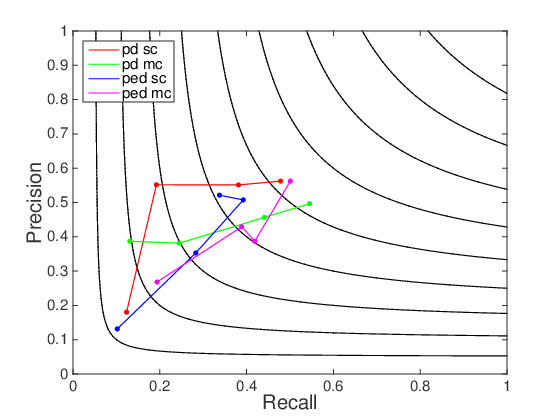
\includegraphics[width=0.47\linewidth] {evaluation/chairs_3_cast/avg/avg_prec_rec}
   \label{fig:chair_3_cast_plot_avg_stat_a}
}
\subfigure[Cluster Count / F1 Score Plot]{
   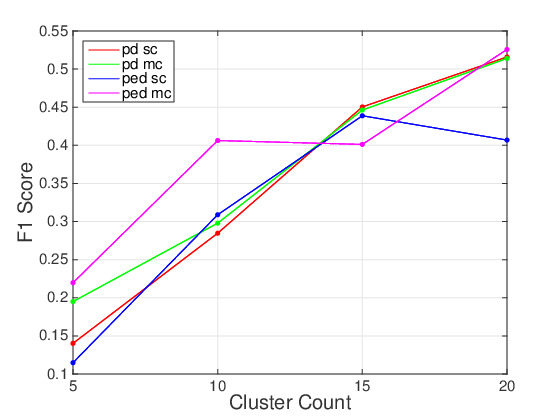
\includegraphics[width=0.47\linewidth] {evaluation/chairs_3_cast/avg/avg_clust_f1}
   \label{fig:chair_3_cast_plot_avg_stat_b}
}
\end{center}
\caption[Chair 3 Cast avg statistic plots]{Plots of the average performance of the four methods PED SC, PD MC, PED SC and PED MC for a varying number of clusters. The left plots shows the recall/precision plot and the figure on the right shows the F1 score alongside the number of clusters. The actual measurements are listed in Table $\ref{tab:chair_3_cast_avg_performance}$.}
\label{fig:chair_3_cast_plot_avg_stat}
\end{figure}

\begin{figure}[H]
\begin{center}
\subfigure[Ground truth frame 60]{
   \includegraphics[width=0.31\linewidth] {evaluation/chairs_3_cast/worst_best/60_amb}
   \label{fig:chair_3_cast_gt_worst_best_a}
}
\subfigure[Worst F1 Score Frame 60]{
   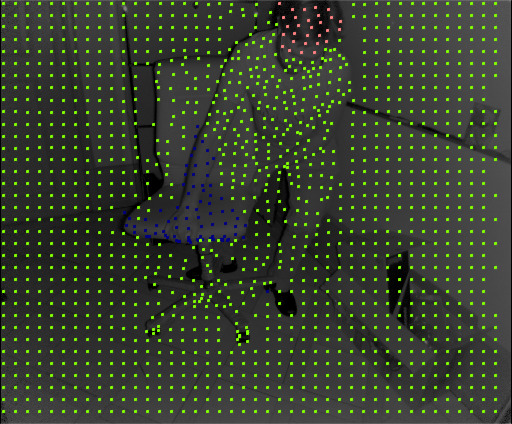
\includegraphics[width=0.31\linewidth] {evaluation/chairs_3_cast/worst_best/ped_sc_c_5_f_60}
   \label{fig:chair_3_cast_gt_worst_best_b}
}
\subfigure[Best F1 Score Frame 60]{
   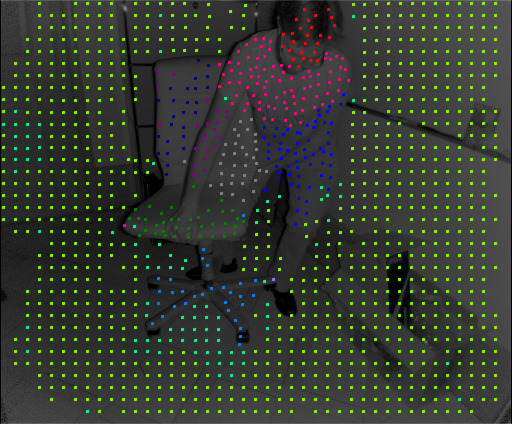
\includegraphics[width=0.31\linewidth] {evaluation/chairs_3_cast/worst_best/ped_mc_c_20_f_60}
   \label{fig:chair_3_cast_gt_worst_best_c}
}
\end{center}
\caption[Chair 3 Cast Worst/Best Result]{Comparison of the worst- (center) and the best (right) segmentation results according to the F1 measure (see Tab. $\ref{tab:chair_3_cast_avg_performance}$) using the shown mask on the left.}
\label{fig:chair_3_cast_gt_worst_best}
\end{figure}